\documentclass[a4paper,12pt]{article}
\usepackage{lmodern}
\usepackage{url}
\usepackage{float}
\usepackage{enumitem}
\usepackage{tabularx}
\usepackage{graphicx}
\usepackage{tikz}
\usepackage{amsmath}
\usepackage[ruled,vlined]{algorithm2e}
\usepackage{listings}
\usepackage{color}

\begin{document}

\begin{titlepage}

\begin{figure}[H]
  \centering
  
\includegraphics[width=8cm]{../stfx_logo.png}\\
  \vspace{1cm}
  {\scshape\Large CSCI - 525: Machine Learning Design \\}
  \vspace{0.5cm}
  {\large Dr. Jacob Levman \\}
  \vspace{1cm}
  {\Large Phase 3 Report \\}
  \vspace{1.8cm}
  {\large Khan, Salal Ali\\ \texttt{202307216 - x2023flb@stfx.ca} \\}
  \vspace{0.5cm}
  {\large Hussain, Moayadeldin\\ \texttt{202407556 - x2024ghl@stfx.ca} \\}
  \vspace{0.5cm}
  {\large Javed, Muhammad\\ \texttt{202303808 - x2023dvh@stfx.ca} \\}
  \vfill
  \vspace{0.5cm}
  {\large Oct 20, 2024 \\}
\end{figure}

\end{titlepage}

\section*{Introduction}

We are currently analyzing Airbnb's 2023 New York City dataset and are using machine learning to predict property prices. The real estate industry is critical for economic development and society progress, reflecting the aspirations of people, families and the overall social health of the region [1]. In the past, knowing property prices relied heavily on human experience and conventional methods. However, these approaches usually did not manage to success to account for the complexity and non-linear relationships of housing market data. With machine learning advancements, the scene has changed with the ability to extract precious information from large volumes of data [2]. Addressing the challenges, predicting house prices accurately remains demanding due to the multitude of influencing factors, as location, size, house quality, condition, etc. [3]. We are looking forward in our work to acquire knowledge from the literature of different models used and address the existing challenges in such problem.

One of the most interesting research work we found on utilizing AI in Airbnb datasets price prediction was founded in [4] by Stanford Researchers. They used plenty of models to address their target, including Ridge Regression, K-means Clustering, Support Vector Regression, Neural Networks and Gradient Boosting Tree Ensemble. They also used Feature Selection and Sentiment Analysis. Sentiment Analysis refers to the application of natural language processing to identify and classify subjective opinions in source materials (e.g., a document or a sentence) [5]. However, this topic is beyond our scope in our Project 1 at the course becauase it depends on transforming the words and sentences to a different feature space using a technique called word embeddings, as Word2Vec [6]. Moreover, the work in [7] focused also on Predicting Airbnb Listing Price with multiple models, utilizing Boston Airbnb open data set from Kaggle, which includes 3, 585 listings between 2016 and 2017. They used Linear Regression, K-nearest neighbor regression and Gradient Boosting regression. The authors in [3] depended on using Linear Regression, and Random Forests. In [2], Linear Regression, Random Forest Regression and Gradient Boosting Regression.

In [4], their experiments involved Mean absolute error (MAE), mean squared error (MSE) and R2 score were used to evaluate their training models. Among the models tested, Support Vector Regression performed the best and produced 69\% R2 score, 0.147 MSE on test split, and 0.2132 on MAE. In [3], the Random Forest Regressor model had high accuracy store with 97.3\% for training set and 82.3\% for the testing set, in comparison with the linear regression model with only 79.4\% and 58.9\% for training and testing. Hence, the authors concluded that the Random Regression model is the best model for study. In [2], they used MAE, RMSE and R2 Score, mostly similar to work in [4], as performance metrics. The authors in [2] found that R2 scores in their work exceeds that in [4] for two models of the three they used, achieving 0.822 and 0.828 with both Random Forest and Gradient Boosting repsectively.

We hypothesize that the use of open source machine learning software applied to New York AirBnb's 2023 dataset may produce useful technology for House Prices prediction and analysis. We hypothesize that applying different Machine Learning, and Preprocessing technqiues, according also to our discussions with Dr. Jacob, will yield to improvements in property price and minimum nights.

\section*{Methods}

In this methods section, we present our methodology in data preprocessing,
analyzing prices and minimum nights, and how to utilize different encoding techniques and correlation between attributes to optimize our results.
The original dataset contains 42,931 records and 18 features as shown in Table \ref{tab:dataframe_overview}

\begin{table}[h!]
\centering
\begin{tabular}{|c|l|l|l|}
\hline
\textbf{\#} & \textbf{Column} & \textbf{Non-Null Count} & \textbf{Dtype} \\ \hline
0 & id & 42931 non-null & int64 \\ \hline
1 & name & 42919 non-null & object \\ \hline
2 & host\_id & 42931 non-null & int64 \\ \hline
3 & host\_name & 42926 non-null & object \\ \hline
4 & neighbourhood\_group & 42931 non-null & object \\ \hline
5 & neighbourhood & 42931 non-null & object \\ \hline
6 & latitude & 42931 non-null & float64 \\ \hline
7 & longitude & 42931 non-null & float64 \\ \hline
8 & room\_type & 42931 non-null & object \\ \hline
9 & price & 42931 non-null & int64 \\ \hline
10 & minimum\_nights & 42931 non-null & int64 \\ \hline
11 & number\_of\_reviews & 42931 non-null & int64 \\ \hline
12 & last\_review & 32627 non-null & object \\ \hline
13 & reviews\_per\_month & 32627 non-null & float64 \\ \hline
14 & calculated\_host\_listings\_count & 42931 non-null & int64 \\ \hline
15 & availability\_365 & 42931 non-null & int64 \\ \hline
16 & number\_of\_reviews\_ltm & 42931 non-null & int64 \\ \hline
17 & license & 1 non-null & object \\ \hline
\end{tabular}
\caption{NYC AirBnb 2023 Dataset Information}
\label{tab:dataframe_overview}
\end{table}

The first step to preprocess our dataset was to remove columns that we may consider as redundant or would degrade the performance of our model, becuase of their irrelevancy treating it as noise, or because they wouldn't give too much information according to the discussion we had with Dr. Jacob Levman during his office hours sharing thoughts about the project.

Hence, we decided to drop \textit{`host\_id, host\_name, last\_review, reviews\_per\_month, calculated\_host\_listings\_count, number\_of\_reviews\_ltm, license'} attributes.

It is implemented also in the code a function called `gettingInsights()' which prints out the number of unique elements in `neighbourhood, neighbourhood\_group, room\_type' attributes. Moreover, it prints out the unique elements in the last two aforementioned attributes.

As mentioned in the project proposal, our first two main goals is to predict the minimum number of nights one user may spend in one apartment, and also the prices. In order to achieve that with higher accuracy, we decided to remove what we considered as `outliers' during our data exploration, these outliers would be defined as:

\begin{enumerate}
    \item Prices: We found out there are 27 records having the label price "zero". We consider this as noise and practically unachievable because basically no one would rent their property in real life for free (unless there are some relationship between the landlord and the tenant that we wouldn't be able to figure out from our features, and something out of the scope and focus of our work.) So we decided to remove all these 27 records.

    \item Minimum Nights: We defined outliers as the number of of nights that appear only once. This means we retain all records where the minimum nights value is repeated at least twice. During our exploration, we found out 7,946 records falling under this criteria. Hence, we decided to remove them.
\end{enumerate}

After cleaning the dataset, the number of records left reduced to 34,977 records, which indicates basically that many houses that were given the label price "zero" had a minimum nights stay number that was repeated only once, we consider this as another indication of them being truly outliers. The distribution of Minimum Nights attributes after removing the outliers defined in (2) below is shown as in Figure \ref{histo}. \newline

\begin{figure}[!t]
\centering
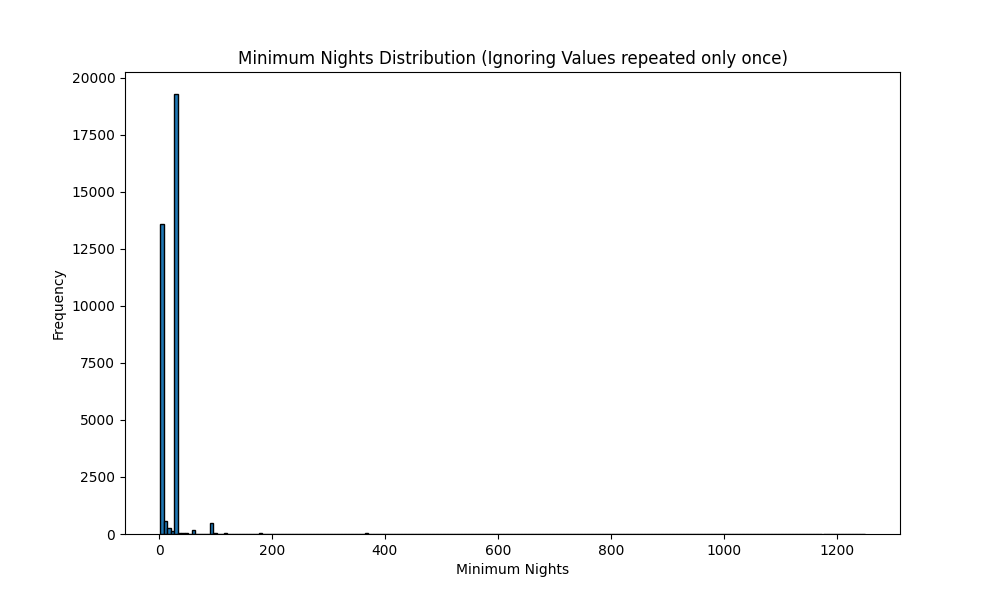
\includegraphics[width=5.5in]{fig.png}
\caption{Histogram showing the frequency of Minimum Nights values after preprocessing}
\label{histo}
\end{figure}


Another main point in the target of our work is to apply different types of Encodings and Natural Language Processing techniques to see how they may enhance the performance, in our implementation, we choose to apply Label Encoding, One Hot Encoding and Bag of Words technique.

After our discussions with Dr. Jacob, we decided to use Label Encoding technique on the \textit{`neighbourhood\_group'} feature, as the feature with the largest number of unique values, it is convenient to label encode it to avoid dimensionality increasing. In Table \ref{tab:neighbourhood_label_encoded}, the top 5 most frequent labels are shown. It is obvious that for example Bedford-Stuyvesant and Williamsburg are by considerable far the most frequent neighbourhoods in the dataset.

\begin{table}[h!]
\centering
\begin{tabular}{|c|c|}
\hline
\textbf{Label Encoded Neighbourhood} & \textbf{count} \\ \hline
12 (Bedford-Stuyvesant) & 2668 \\ \hline
216 (Williamsburg) & 2385 \\ \hline
96 (Harlem) & 1806 \\ \hline
27 (Cambria Heights) & 1570 \\ \hline
129 (Midtown) & 1407 \\ \hline
\end{tabular}
\caption{Top-5 Most Frequent Label Encoded Values}
\label{tab:neighbourhood_label_encoded}
\end{table}

Regarding the One Hot Encoding, when we say we store one-hot encoded values directly, we refer to saving an actual one or zero for each element of a vector [8]. We decided we are going to encode both the \textit{`neighbourhood\_group' } and `room\_type'. There are 5 Neighbourhood Group Set Elements which are `Queens', `Manhattan', `Staten Island', `Bronx', `Brooklyn'. Moreover, there are 4 Room Type Set Elements which are `Entire home/apt', `Shared room', `Hotel room', `Private room'. Each of these attributes were used resulting in adding 9 additional features to the dataset, each one represents OHE for the specific attribute. \newline

On the Bag of Words technique, we consider our implementation in this area a contribution in this type of work. The bag of words (BOW) method can be employed to treat each remaining word as a feature of the document [9]. According to our discussions with Dr. Jacob, we needed to determine the most relevant words in the names of properties. In order to do so, the literature review in this area usually focus on using some kind of Word Embedding technique to handle such case. However, we thought that in this Project 1 work we may address it in a different, easier and much innovative way.

We decided to pick up the top 100 frequent words in our name column and check for the words that has high correlation with the price feature, we put a threshold of positive/negative correlation (+/-0.02) in order to determine whether this word is relevant or not, we used Pearson's correlation coefficient. Correlation coefficients are utilized to evaluate the strength and direction of linear relationships between variables pairs. [10]. Our approach returned eight different words with highest correlation which were `luxury', `hotel', `floor', `city', `private', `in', `cozy', `room'. Afterwards, we applied One Hot Encoding to make each occurrence of a word in a record counts, and finally, we append the result of the encoding to the dataframe as columns.

\section*{Results}

In Phase 2, we ran df-Analyze only once on one target feature, which was the price. Moreover, we have performed Label Encoding, One Hot Encoding and dropping the redundant features.

In Phase 3, We ran df-Analyze four times. The first two runs focused on predicting the target Minimum Nights and Price features separately, following the full data preprocessing guideline described in Section 3. Additionally, the third and fourth runs aimed to predict the same target features, but this time after removing the number\_of\_reviews feature. This suggestion comes from Dr. Jacob suggestion he offered in the feedback we received on Phase 2 results, which can be interpreted also from Table \ref{table_preprocessing_phases}.

We compare the results from Phase 2 of the df-Analyze run, which we dedicated on predicting the price feature, with the outcomes from two runs in Phase 3, where we predicted the price feature once including the number\_of\_reviews feature and once without. We evaluate the performances on the holdout set. The privilege of using df-Analyze [11] is that it allows us to explore such models with different types of data embeddings. Hence, we introduce some of the models for comparison purposes and full results is uploaded among this project's materials. The models we will introduce are LGBM (Light Gradeint-Boosting Machine) with linear embeddings, SGD (Stochastic Gradient Descent) with association, and RF (Random Forest) with pred selection. Moreover to remain consistent with other works provided in the literature, we will refer to Mean Absolute Error (MAE), Mean Squared Error (MSE), and R2 score as our performance metrics.

\begin{table}[h!]
\centering
\begin{tabular}{|c|p{10cm}|}
\hline
\textbf{Phase Number} & \textbf{Preprocessing Steps} \\ \hline
Phase 2 & Label Encoding, One Hot Encoding, Removing Redundant Features. \\ \hline
Phase 3 & Label Encoding, One Hot Encoding, Removing Redundant Features, Implementing Bag of Words with Applying Pearson Correlation, Removing outliers from Minimum Nights and Prices, Trying to figure out whether removing `number of reviews' feature can enhance the results. \\ \hline
\end{tabular}
\caption{Comparing Preprocessing Steps for Phases 2 and 3}
\label{table_preprocessing_phases}
\end{table}

\begin{table}[h!]
    \centering
    \resizebox{\textwidth}{!}{%
    \begin{tabular}{|c|c|c|c|c|}
        \hline
        \textbf{Phase Number} & \textbf{MAE} & \textbf{MSE} & \textbf{R2} & \textbf{Method} \\
        \hline
        Phase 2 & 0.163 & 1.664 & -0.016 & LGBM Embed-Linear \\
        Phase 3 & \textbf{0.150} & \textbf{0.239} & 0.065 & LGBM Embed-Linear \\
        Phase 3 with removing Number of Reviews & 0.158 & 0.849 & \textbf{0.074} & LGBM Embed-Linear \\
        \hline
        Phase 2 & 0.159 & 1.608 & 0.018 & RF Pred \\
        Phase 3 & \textbf{0.152} & \textbf{0.235} & 0.079 & RF Pred \\
        Phase 3 with removing Number of Reviews & 0.156 & 0.838 & \textbf{0.086} & RF Pred \\
        \hline
        Phase 2 & 0.154 & 1.633 & 0.002 & SGD Assoc \\
        Phase 3 & \textbf{0.149} & \textbf{0.242} & 0.052 & SGD Assoc \\
        Phase 3 with removing Number of Reviews & 0.152 & 0.831 & \textbf{0.094} & SGD Assoc \\
        \hline
    \end{tabular}%
    }
    \caption{df-Analyze Results of Predicting Price Feature}
    \label{tab:df_analyze_predicting_price}
\end{table}

The results are shown in Table \ref{tab:df_analyze_predicting_price}. It is clear that our innovative approach of introducing Bag of Words with Pearson's Correlation coefficient, along with removing Prices and Minimum Nights outliers have significantly improved the performance. It is also obvious that removing `number\_of\_reviews' feature didn't improve the loss percentages. However, it has impacted the R2 score with making it getting higher in the three models.

It is difficult to compare our model's performances with other literature review mentioned in the introduction, as we aren't working on the same datasets or on a common benchmark ones where we can evaluate on the same baseline. However, we provide an analogy with the results in [4] just for illustrative reasons. In [4] they used the same 3 performance measures we have used in our analysis (MAE, MSE, R2 Score). The authors best model's performance achieved 0.147 MSE error on the test set. We achieve comparable performance of 0.239 and 0.235 with our two best models, LGBM and Random Forests respectively. Moreover, they achieve 0.2132 as MAE. Our df-Analyze best MAE perofrmances are 0.150 and 0.149 with LGBM and SGD respectively.

Regarding predicting Minimum Nights, we also compare the results from Phase 3 without removing number of reviews, and Phase 3 with removing number of reviews feature, as we didn't run df-analyze on Minimum Nights as a target in Phase 2. From the results shown in Table \ref{tab:df_analyze_predicting_nights}, it is clear that LGBM performs better when `number\_of\_reviews' features is removed. On the other hand, it is also clear that SGD performs better when this feature is kept among the dataset. Random Forests MAE loss was better with the feature's presence, and MSE and R2 values were better with the feature's absence.

\begin{table}[h!]
    \centering
    \resizebox{\textwidth}{!}{%
    \begin{tabular}{|c|c|c|c|c|}
        \hline
        \textbf{Phase Number} & \textbf{MAE} & \textbf{MSE} & \textbf{R2} & \textbf{Method} \\
        \hline
        Phase 3 & 0.195 & 0.241 & 0.119 & LGBM Embed-Linear \\
        Phase 3 without Number of Reviews & \textbf{0.187} & \textbf{0.181} & \textbf{0.231} & LGBM Embed-Linear \\
        \hline
        Phase 3 & \textbf{0.194} & 0.246 & 0.100 & RF Pred \\
        Phase 3 without Number of Reviews & 0.195 & \textbf{0.206} & \textbf{0.126} & RF Pred \\
        \hline
        Phase 3 & \textbf{0.230} & \textbf{0.274} & \textbf{-0.001} & SGD Assoc \\
        Phase 3 without Number of Reviews & 0.243 & 0.276 & -0.156 & SGD Assoc \\
        \hline
    \end{tabular}%
    }
    \caption{df-Analyze Results of Predicting Minimum Nights}
    \label{tab:df_analyze_predicting_nights}
\end{table}

We can deduce from the results that our further preprocessing in Phase 3 made a huge enhancement in the results compared to Phase 2 in properties price predictions, which shows the robustness of our approach. Moreover, removing `number\_of\_reviews' attribute as per Dr. Jacob suggestion seems to have a negative impact on the losses of prices predictions, but it improves the R2 score. We have shown also from the illustration of our results that our method is competent with other similar and proven work in the literature. Regarding predicting Minimum Nights, we compared both of our Phase 3 runs on this target attribute and it was shown that removing `number\_of\_reviews' attributes may likely produce an enhancment in some models performances.


\newpage
\sloppy
\section*{References}
\begin{enumerate}
  \item Li, Chenxi. (2024). House price prediction using machine learning. Applied and Computational Engineering. 53. 225-237. 10.54254/2755-2721/53/20241426.
  \item el Mouna, Lale \& Hassan, Silkan \& Haynf, Youssef \& Nann, Mohamedade \& Koumetio Tekouabou, Cédric Stéphane. (2023). A Comparative Study of Urban House Price Prediction using Machine Learning Algorithms. E3S Web of Conferences. 418. 10.1051/e3sconf/202341803001.
  \item Maloku, Fatbardha. (2024). House Price Prediction Using Machine Learning and Artificial Intelligence. Journal of Artificial Intelligence \& Cloud Computing. Volume 3(4): 1- 10. 1-10. 10.47363/JAICC/2024(3)357.
  \item Rezazadeh Kalehbasti, P., Nikolenko, L., Rezaei, H. (2021). Airbnb Price Prediction Using Machine Learning and Sentiment Analysis. In: Holzinger, A., Kieseberg, P., Tjoa, A.M., Weippl, E. (eds) Machine Learning and Knowledge Extraction. CD-MAKE 2021. Lecture Notes in Computer Science(), vol 12844. Springer, Cham. https://doi.org/10.1007/978-3-030-84060-0\_11
  \item Luo, Tiejian \& Chen, Su \& Xu, Guandong \& Zhou, Jia. (2013). Sentiment Analysis. 10.1007/978-1-4614-7202-5\_4.
  \item Mikolov, Tomas \& Kai, Chen \& Corrado,Greg and Dean, Jeffrey. (2013). Efficient Estimation of Word Representations in Vector Space. https://arxiv.org/abs/1301.3781
  \item Wang, Haoqian. (2023). Predicting Airbnb Listing Price with Different models. Highlights in Science, Engineering and Technology. 47. 79-86. 10.54097/hset.v47i.8169.
  \item Hancock, J.T., Khoshgoftaar, T.M. Survey on categorical data for neural networks. J Big Data 7, 28 (2020). https://doi.org/10.1186/s40537-020-00305-w
  \item Juluru K, Shih HH, Keshava Murthy KN, Elnajjar P. Bag-of-Words Technique in Natural Language Processing: A Primer for Radiologists. Radiographics. 2021 Sep-Oct;41(5):1420-1426. doi: 10.1148/rg.2021210025. Epub 2021 Aug 13. PMID: 34388050; PMCID: PMC8415041.
  \item Mukaka MM. Statistics corner: A guide to appropriate use of correlation coefficient in medical research. Malawi Med J. 2012 Sep;24(3):69-71. PMID: 23638278; PMCID: PMC3576830.
  \item df-Analyze: https://github.com/stfxecutables/df-analyze
\end{enumerate}


\end{document}
